%
% 43-pole.tex -- Ein Beispiel ohne Pole
%
% (c) 2026 Prof Dr Andreas Müller
%
\subsection{Ein Beispiel ohne Pole}
%
% fig-ecos.tex
%
% (c) 2026 Prof Dr Andreas Müller
%
\begin{figure}
\centering
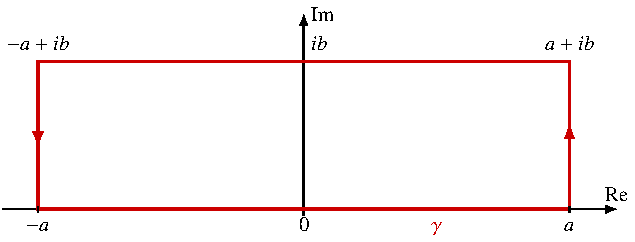
\includegraphics{chapters/030-integration/images/ecos.pdf}
\caption{Weg zur Auswertung des Integrals
$\int_{-\infty}^\infty \cos 2bx \cdot e^{-x^2}\,dx$.
\label{buch:integration:residuen:fig:ecos}}
\end{figure}
%
Die Funktion $f(z)=e^{-z^2}$ ist holomorph in der ganzen komplexen 
Ebene, für jeden beliebigen geschlossenen Weg gilt daher nach dem
Satz~\ref{buch:integration:wegintegral:satz:cauchy}
von Cauchy
\begin{equation}
\int_{\gamma} e^{-z^2}\,dz
=
0.
\label{buch:integration:residuen:eqn:wegintegral}
\end{equation}
Die Funktion $e^{-z^2}$ ist bekannt dafür, dass sie keine elementare
Stammfunktion hat.
Da sie aber in der Wahrscheinlichkeitsdichte der Normalverteilung
vorkommt, sind Integrale dieser Funktion von einiger praktischer
Bedeutung.

Das uneigentliche Integral
\index{Integral!uneigentlich}%
\[
\int_{-\infty}^{\infty} e^{-x^2}\,dx = \!\sqrt{\pi}
\]
kann mithilfe eines zweifachen Integrals bestimmt werden, wir nehmen
es hier als bekannt an.

Wir betrachten jetzt das Integral entlang des rechteckigen Weges $\gamma$
in Abbildung~\ref{buch:integration:residuen:fig:ecos}.
Das Integral über den unteren Rand des Rechtecks ist
\[
\int_{-a}^a
e^{-x^2}
\,dx
\to
\!\sqrt{\pi}
\]
für $a\to\infty$.
Wegen~\eqref{buch:integration:residuen:eqn:wegintegral}
müssen die verbleibenden Teile des Weges den Wert $-\!\sqrt{\pi}$ ergeben.
Wir berechnen diese Teile.

Die vertikalen Teile des Weges haben die Form
\begin{align*}
\int_0^b
e^{-(a+iy)^2}
\cdot i
\,dy
&=
i
e^{-a^2}
\int_0^b
e^{y^2 -2iby}
\,dy
\intertext{mit Betrag}
\biggl|
\int_0^b
e^{-(a+iy)^2}
\cdot i
\,dy
\biggr|
&=
e^{-a^2}
\biggl|
\int_0^b
e^{y^2 -2iby}
\,dy
\biggr|
\\
&\le
e^{-a^2}
\int_0^b
\bigl|e^{y^2 -2iby}\bigr|
\,dy
=
e^{-a^2}
\int_0^b
e^{y^2}
\,dy
\le
e^{-a^2}be^{b^2}.
\end{align*}
Die rechte Seite konvergiert gegen $0$, wenn $a\to\infty$.
Im Grenzwert $a\to\infty$ tragen die vertikalen Teile des Weges
also nichts bei.

Wir können jetzt schliessen, dass im Grenzwert $a\to\infty$ sich die
Integrale über den oberen und unter Rand wegheben.
Das Integral über den oberen Rand des Rechtecks ist
\begin{align*}
\int_{a}^{-a}
e^{-(x+ib)^2}
\,dx
&=
\int_{a}^{-a}
e^{-x^2+b^2-2ixb}
\,dx
=
e^{b^2}
\int_{a}^{-a}
e^{-x^2}
\bigl(
\cos(2bx) - i\sin(2bx)
\bigr)
\,dx
\\
&=
e^{b^2}
\int_{a}^{-a}
e^{-x^2}
\cos(2bx)
\,dx
-i
e^{b^2}
\int_{a}^{-a}
e^{-x^2}
\sin(2bx)
\,dx.
\end{align*}
Das zweite Integral hat einen ungeraden Integranden, wird aber über
ein symmetrisches Interval erstreckt, daher verschwindet es.
Im Grenzwert $a\to\infty$ gilt
\begin{align*}
\!\sqrt{\pi}
+
e^{b^2}
\int_{\infty}^{-\infty}
e^{-x^2}
\cos(2bx)
\,dx
&=
0
\\
\!\sqrt{\pi}
&=
e^{b^2}
\int_{-\infty}^{\infty}
e^{-x^2}
\cos(2bx)
\,dx
\intertext{oder}
\int_{-\infty}^{\infty}
e^{-x^2}
\cos(2bx)
\,dx
&=
\!\sqrt{\pi}e^{-b^2}.
\end{align*}
Man beachte, dass das Integral nicht mit der traditionellen Methode
der Stammfunktion berechnet werden kann.
Wie für den Integranden $e^{-x^2}$ kann auch für den Integranden
$\cos(2bx)e^{-x^2}$ kein Stammfunktion in geschlossener Form
gefunden werden.
Die Methode der Wegintegrale in der komplexen Ebene ist also die
einzige Methode, dieses Integral exakt zu berechnen.
